\documentclass{article}

% packages
\usepackage{amsmath, amsthm, thmtools, amsfonts, amssymb, luacode, catchfile, tikzducks, hyperref, ifthen}
\ifcsname c@kobocompile\endcsname
	\usepackage[a5paper, total={1072pt, 1448pt}, margin=10pt, includeheadfoot]{geometry} % set page margins
\else
	\usepackage[a4paper, margin=50pt, includeheadfoot]{geometry}
\fi
\usepackage[shortlabels]{enumitem}
\usepackage[skip=3pt, indent=0pt]{parskip}

% language
\usepackage[bidi=basic, layout=tabular, provide=*]{babel}
\ifcsname c@english\endcsname
	\babelprovide[main, import]{english}
\else
	\babelprovide[main, import]{hebrew}
	\babelprovide{rl}
\fi
%\babelfont{rm}{Libertinus Serif}
\babelfont{rm}[Renderer=Harfbuzz]{Libertinus Serif}
\babelfont{sf}{Libertinus Sans}
\babelfont{tt}{Libertinus Mono}

% style
\AddToHook{cmd/section/before}{\clearpage}	% Add line break before section
\linespread{1.3}
\setcounter{secnumdepth}{0}		% Remove default number tags from sections, this won't do well with theorems
\AtBeginDocument{\setlength{\belowdisplayskip}{3pt}}
\AtBeginDocument{\setlength{\abovedisplayskip}{3pt}}
\graphicspath{ {../images/} }

% operators
\DeclareMathOperator\cis{cis}
\DeclareMathOperator\Sp{Sp}
\DeclareMathOperator\tr{tr}
\DeclareMathOperator\im{Im}
\DeclareMathOperator\re{Re}
\DeclareMathOperator\diag{diag}
\DeclareMathOperator*\lowlim{\underline{lim}}
\DeclareMathOperator*\uplim{\overline{lim}}
\DeclareMathOperator\rng{rng}
\DeclareMathOperator\Sym{Sym}
\DeclareMathOperator\Arg{Arg}
\DeclareMathOperator\Log{Log}
\DeclareMathOperator\dom{dom}
\DeclareMathOperator\supp{Supp}
\DeclareMathOperator\var{Var}
\DeclareMathOperator\cov{Cov}

% commands
%\renewcommand\qedsymbol{\textbf{מש''ל}}
%\renewcommand\qedsymbol{\fbox{\emoji{lizard}}}
\newcommand{\Aa}[0]{\mathcal{A}}
\newcommand{\Bb}[0]{\mathcal{B}}
\newcommand{\CC}[0]{\mathbb{C}}
\newcommand{\Cc}[0]{\mathcal{C}}
\newcommand{\EE}[0]{\mathbb{E}}
\newcommand{\FF}[0]{\mathbb{F}}
\newcommand{\Ff}[0]{\mathcal{F}}
\newcommand{\Ii}[0]{\mathcal{I}}
\newcommand{\Gg}[0]{\mathcal{G}}
\newcommand{\Ll}[0]{\mathcal{L}}
\newcommand{\Mm}[0]{\mathcal{M}}
\newcommand{\NN}[0]{\mathbb{N}}
\newcommand{\Nn}[0]{\mathcal{N}}
\newcommand{\PP}[0]{\mathbb{P}}
\newcommand{\Pp}[0]{\mathcal{P}}
\newcommand{\QQ}[0]{\mathbb{Q}}
\newcommand{\RR}[0]{\mathbb{R}}
\newcommand{\Rr}[0]{\mathcal{R}}
\newcommand{\Ss}[0]{\mathcal{S}}
\newcommand{\TT}[0]{\mathbb{T}}
\newcommand{\Uu}[0]{\mathcal{U}}
\newcommand{\Vv}[0]{\mathcal{V}}
\newcommand{\Ww}[0]{\mathcal{W}}
\newcommand{\ZZ}[0]{\mathbb{Z}}
\newcommand{\acts}[0]{\circlearrowright}
\newcommand{\explain}[2] {
	\begin{flalign*}
		 && \text{#2} && \text{#1}
	\end{flalign*}
}
\newcommand{\maketitleprint}[0]{ \begin{center}
	%\begin{tikzpicture}[scale=3]
	%	\duck[graduate=gray!20!black, tassel=red!70!black]
	%\end{tikzpicture}	
	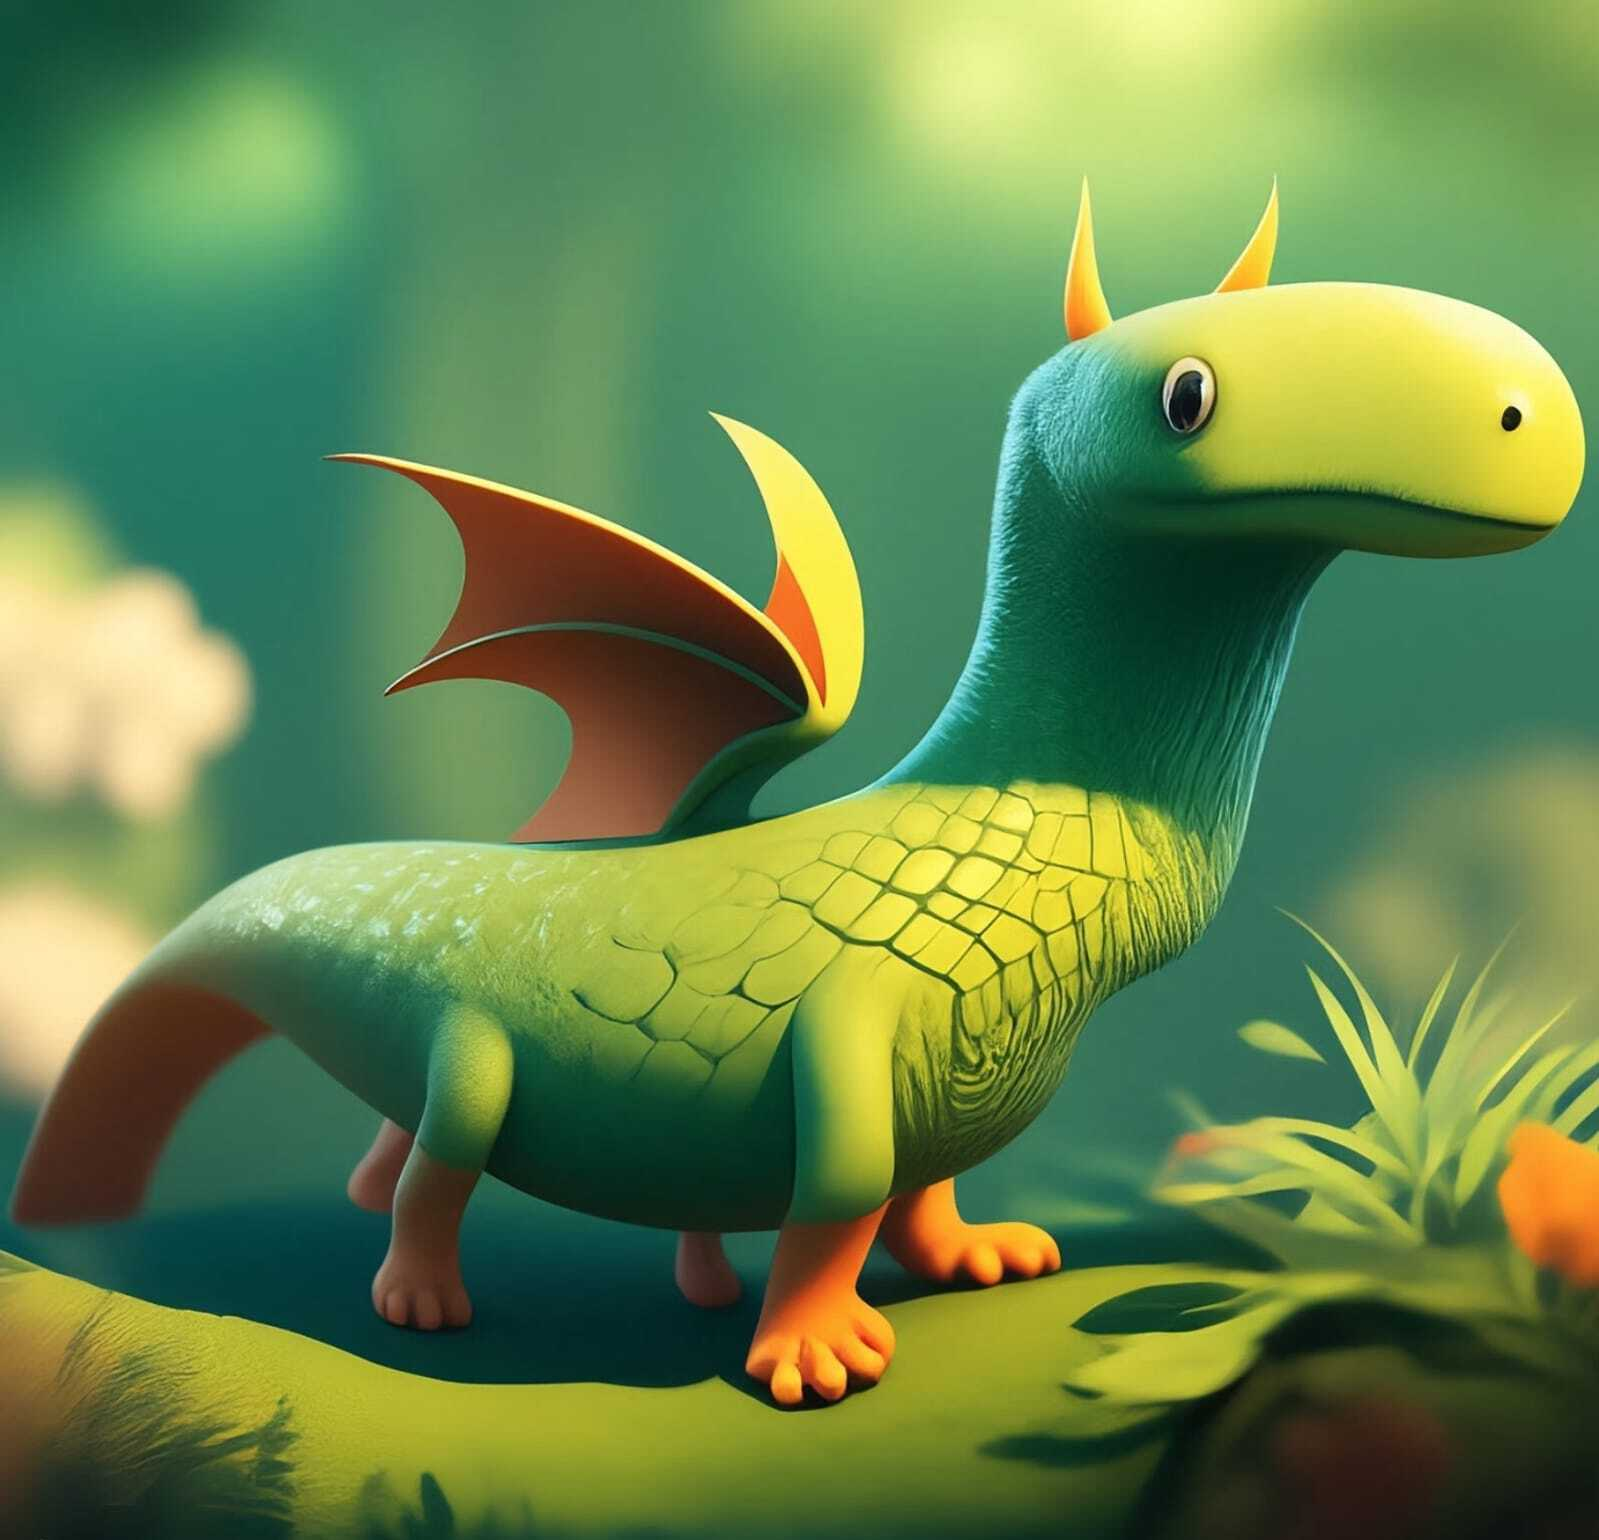
\includegraphics[width=6cm]{cover}
\end{center}
}

% theorem commands
\newtheoremstyle{c_remark}
	{}	% Space above
	{}	% Space below
	{}% Body font
	{}	% Indent amount
	{\bfseries}	% Theorem head font
	{}	% Punctuation after theorem head
	{.5em}	% Space after theorem head
	{\thmname{#1}\thmnumber{ #2}\thmnote{ \normalfont{\text{(#3)}}}}	% head content
\newtheoremstyle{c_definition}
	{3pt}	% Space above
	{3pt}	% Space below
	{}% Body font
	{}	% Indent amount
	{\bfseries}	% Theorem head font
	{}	% Punctuation after theorem head
	{.5em}	% Space after theorem head
	{\thmname{#1}\thmnumber{ #2}\thmnote{ \normalfont{\text{(#3)}}}}	% head content
\newtheoremstyle{c_plain}
	{3pt}	% Space above
	{3pt}	% Space below
	{\itshape}% Body font
	{}	% Indent amount
	{\bfseries}	% Theorem head font
	{}	% Punctuation after theorem head
	{.5em}	% Space after theorem head
	{\thmname{#1}\thmnumber{ #2}\thmnote{ \text{(#3)}}}	% head content

\ifcsname c@english\endcsname
	\theoremstyle{plain}
	\newtheorem{theorem}{Theorem}[section]
	\newtheorem{lemma}[theorem]{Lemma}
	\newtheorem{proposition}[theorem]{Proposition}
	\newtheorem*{proposition*}{Proposition}
	%\newtheorem{corollary}[theorem]{אין חלופה עברית}

	\theoremstyle{definition}
	\newtheorem{definition}[theorem]{Definition}
	\newtheorem*{definition*}{Definition}
	\newtheorem{example}{Example}[section]
	\newtheorem{exercise}{Exercise}[section]

	\theoremstyle{remark}
	\newtheorem*{remark}{Remark}
	\newtheorem*{solution}{Solution}
	\newtheorem{conclusion}[theorem]{Conclusion}
	\newtheorem{notation}[theorem]{Notation}
\else
	\theoremstyle{c_plain}
	\newtheorem{theorem}{משפט}[section]
	\newtheorem{lemma}[theorem]{למה}
	\newtheorem{proposition}[theorem]{טענה}
	\newtheorem*{proposition*}{טענה}
	%\newtheorem{corollary}[theorem]{אין חלופה עברית}

	\theoremstyle{c_definition}
	\newtheorem{definition}[theorem]{הגדרה}
	\newtheorem*{definition*}{הגדרה}
	\newtheorem{example}{דוגמה}[section]
	\newtheorem{exercise}{תרגיל}[section]

	\theoremstyle{c_remark}
	\newtheorem*{remark}{הערה}
	\newtheorem*{solution}{פתרון}
	\newtheorem{conclusion}[theorem]{מסקנה}
	\newtheorem{notation}[theorem]{סימון}
\fi

% Questions related commands
\newcounter{question}
\setcounter{question}{1}
\newcounter{sub_question}
\setcounter{sub_question}{1}

\ifcsname c@english\endcsname
	\newcommand{\question}[1][0]{
		\ifthenelse{#1 = 0}{}{\setcounter{question}{#1}}
		\section{Question \arabic{question}}
		\addtocounter{question}{1}
		\setcounter{sub_question}{1}
	}

	\newcommand{\subquestion}[1][0]{
		\ifthenelse{#1 = 0}{}{\setcounter{sub_question}{#1}}
		\subsection{Part \alph{sub_question}}
		\addtocounter{sub_question}{1}
	}
\else
	\newcommand{\question}[1][0]{
		\ifthenelse{#1 = 0}{}{\setcounter{question}{#1}}
		\section{שאלה \arabic{question}}
		\addtocounter{question}{1}
		\setcounter{sub_question}{1}
	}

	\newcommand{\subquestion}[1][0]{
		\ifthenelse{#1 = 0}{}{\setcounter{sub_question}{#1}}
		\subsection{סעיף \localecounter{letters.gershayim}{sub_question}}
		\addtocounter{sub_question}{1}
	}
\fi

% import lua and start of document
\directlua{common = require ('../common')}

\GetEnv{AUTHOR}

% headers
\author{\AUTHOR}
\date\today

\title{פתרון מטלה 10 --- מבנים אלגבריים (2), 80446}

\begin{document}
\maketitle
\maketitleprint[red]

\question{}
יהי $f \in \QQ[x]$ פולינום אי־פריק מדרגה 3 ויהי $L$ שדה הפיצול שלו. \\
נראה ש־$[L : \QQ] = 3$ אם ורק אם $D_f$ ריבוע ב־$\QQ$, ושאחרת $[L : \QQ] = 6$.
\begin{proof}
	תהי $G = \gal(L / \QQ)$, אז בהכרח $G \le S_3$ וטרנזיטיבית, לכן $G \simeq \ZZ / 3\ZZ$ או $G \simeq S_3$. \\
	אם $[L : \QQ] = 3$ אז $G \simeq \ZZ / 3\ZZ$ ולכן קיים אוטומורפיזם $\sigma \in G$ כך ש־$\langle \sigma \rangle = G$.
	\[
		\sigma(\sqrt{D_f})
		= \prod_{1 \le i < j \le 3} (\sigma(x_i) - \sigma(x_j))
		= \prod_{1 \le i < j \le 3} (x_i - x_j)
		= \sqrt{D_f}
	\]
	כלומר זוהי נקודת שבת של $\sigma$ ולכן $\sqrt{D_f} \in \QQ$.

	נניח ש־$\sqrt{D_f}$ ריבוע ב־$\QQ$.
	נניח גם ש־$\sigma \in S_3 \setminus \ZZ / 3\ZZ$, כלומר $\sigma = (x_1\ x_2)$ בלי הגבלת הכלליות,
	מההנחה שלנו גם,
	\[
		\sigma(\sqrt{D_f})
		= \sqrt{D_f}
	\]
	אבל,
	\[
		\sigma(\sqrt{D_f})
		= \sigma(x_1 - x_2) \sigma(x_1 - x_3) \sigma(x_2 - x_3)
		= (x_2 - x_1) (x_2 - x_3) (x_1 - x_3)
		= - \sqrt{D_f}
	\]
	וזו סתירה, לכן $\sigma \notin G$, ובהכרח רק $G \simeq \ZZ / 3\ZZ$, כלומר $[L : \QQ] = 3$.

	אילו התנאי לא מתקיים, אז $G \simeq S_3$ ולכן,
	\[
		[L : \QQ]
		= |G|
		= |S_3|
		= 6
	\]
	כפי שרצינו.
\end{proof}

\question{}
יהיו $F$ שדה ממציין שונה מ־2, $f \in F[x]$ פולינום ספרבילי אי־פריק ומתוקן, ו־$L$ שדה הפיצול של $f$ מעל $F$.
נסמן ב־$\alpha_1, \ldots, \alpha_n$ את שורשי $f$ ב־$L$ ונגדיר $K = F(\sqrt{D_f})$.
נראה שמתקיים,
\[
	\gal(L / K)
	= \{ \sigma \in \gal(L / F) \mid \operatorname{sgn}(\sigma \restriction \{\alpha_1, \ldots, \alpha_n\}) = 1 \}
\]
כלומר ש־$\gal(L / K) = \gal(L / F) \cap A_n$ עד כדי איזומורפיזם.
\begin{proof}
	בתרגול ראינו כי $G \subseteq A_n \iff \sqrt{D_f} \in F$ לכל שדה $F$.
	לכן $K$ מקיימת $\gal(L / K) \subseteq A_n$, ומהתאמת גלואה בפרט $\gal(L / K) \subseteq \gal(L / F) \cap A_n$.
	נותר אם כן להראות שזהו שוויון. \\
	תהי $\sigma \in (\gal(L / F) \cap A_n) \setminus \gal(L / K)$, כלומר $\sigma \restriction K \ne \id_K$.
	אבל $\sigma(\sqrt{D_f}) = \pm \sqrt{D_f}$ בלבד, ובמקרה זה נקבל $\operatorname{sgn}(\sigma) = -1$ ישירות מהגדרת הסימן, ולכן $\sigma \notin A_n$, ונוכל להסיק שאין $\sigma$ כזו. \\
	בהתאם נסיק $\gal(L / K) = \gal(L / F) \cap A_n$.
\end{proof}

\question{}
יהיו $F$ שדה, $f \in F[x]$ פולינום ספרבילי אי־פריק ומתוקן, ו־$L$ שדה הפיצול של $f$ מעל $F$. \\
נניח גם ש־$p = \operatorname{char} F$ וכן ש־$p = 0$ או שעבור $n = | \gal(L / F) |$ מתקיים $p \nmid n$.
תהי $H \le \gal(L / F)$.

\subquestion{}
נגדיר את ההעתקה הלינארית $A_H : L \to L$ על־ידי,
\[
	A_H(x)
	= \frac{1}{|H|} \sum_{\sigma \in H} \sigma(x)
\]
נראה ש־$A_H$ היא הטלה על $L^H$,
כלומר ש־$\im(A_H) = L^H$ ו־$A_H \restriction L^H = \id_{L^H}$.
\begin{proof}
	תהי $\tau \in H$, אז מתקיים,
	\[
		\tau(A_H(x))
		= \tau(\frac{1}{|H|} \sum_{\sigma \in H} \sigma(x))
		= \frac{1}{|H|} \sum_{\sigma \in \tau H} \sigma(x)
		= \frac{1}{|H|} \sum_{\sigma \in H} \sigma(x)
		= A_H(x)
	\]
	כנביעה מ־$\tau H = H$, שכן חבורות גלואה תמיד טרנזיטיביות.
	נסיק ש־$A_H(x) \in L^H = \{ x \in L \mid \forall \sigma \in H,\ \sigma(x) = x \}$.

	יהי $x \in L^H$, כלומר $\sigma(x) = x$ לכל $\sigma \in H$, לכן,
	\[
		A_H(x)
		= \frac{1}{|H|} \sum_{\sigma \in H} \sigma(x)
		= \frac{1}{|H|} \sum_{\sigma \in H} x
		= \frac{1}{|H|} x \cdot |H|
		= x
	\]
	וקיבלנו ש־$A_H \restriction L^H = \id_{L^K}$.
\end{proof}

\subquestion{}
נסיק שאם $B = (b_1, \ldots, b_n)$ בסיס ל־$L$ מעל $F$ אז $\Sp\{ A_H(b_1), \ldots, A_H(b_n)\} = L^H$.
\begin{proof}
	יהי $x \in L^H$ ונניח שמתקיים,
	\[
		x
		= \sum_{i = 1}^n \alpha_i b_i
	\]
	אז מתקיים גם,
	\[
		x
		= A_H(x)
		= \sum_{i = 1}^n A_H(\alpha_i b_i)
		= \sum_{i = 1}^n \alpha_i A_H(b_i)
	\]
	נובע ש־$\Sp\{ A_H(b_1), \ldots, A_H(b_n)\} \supseteq L^H$.

	מהצד השני אם $x \in \Sp\{ A_H(b_1), \ldots, A_H(b_n)\}$ אז,
	\[
		x
		= \sum_{i = 1}^n \alpha_i A_H(b_i)
		= A_H\left(\sum_{i = 1}^n \alpha_i b_i\right)
		\in L^H
	\]
	מלינאריות $A_H$, ולכן מצאנו שיש שוויון.
\end{proof}

\pagebreak
\subquestion{}
נמצא דוגמה ל־$F, f, L, H$ כמוגדר לעיל, ו־$\alpha \in L$ כך ש־$F(\alpha) = L$ אבל שגם,
\[
	F(A_H(\alpha)) \subsetneq L^H
\]
\begin{solution}
	נגדיר,
	\[
		F = \QQ,
		\quad
		f(x) = x^3 - 2,
		\quad
		\alpha = \xi_3 \sqrt[3]{2},
		\quad
		L = F(\alpha),
		\quad
		L^H = F(\xi_3)
	\]
	נגדיר בהתאמה,
	\[
		H
		= \ZZ / 3\ZZ
		= \{ \xi_3 \to \xi_3^i \mid 0 \le i \le 2 \}
	\]
	ולכן נוכל להסיק,
	\[
		A_H(\alpha)
		= \frac{1}{3} \sum_{\sigma \in H} \sigma(\alpha)
		= \frac{1}{3} \sum_{i = 0}^2 \xi_3^i \sqrt[3]{2}
		= 0
	\]
	ולכן,
	\[
		F(A_H(\alpha))
		= F(0)
		= F
		\subsetneq L
	\]
\end{solution}

\end{document}
